\chapter{Anonymous Communication and Onion Routing}

\section{Problems and Goals}
For safety, we need a technique for routing that protect the identity of the sender and the receiver.

\paragraph{Ideas}
\begin{enumerate}
    \item Nodes that do the type of hop-to-hop routing.
    \item Keys that are needed to decrypt the message (payload, not the header)
    \item New routes. Although we want to utilize the route with keys for a while, we need to switch to a new route.
\end{enumerate}

\paragraph{Weakness}
Attackers can find out the hot spots in the network at certain times. \textbf{Why?} Because if the network is on client/server mode, the traffic will concentrated around the server, which makes it a hot spot. Distributing the servers may help, but as long as clients out numbers the servers, there are always hot spots. The solution to this imbalance is a peer-to-peer architecture. 

\section{Peer-to-Peer}
\paragraph{Why we want to transfer to peer-to-peer mode?}
Because client-server mode make the system more vulnerable to attackers.
\paragraph{Challenge from Peer-to-Peer}
Naming the hosts, Finding the hosts, Trusting the hosts.
\paragraph{Solution to the Challenges}
For naming and finding the hosts:
\begin{enumerate}
    \item distributed directory service.
    \item directory service distributed on selected peers.
    \item distributed hashing.
\end{enumerate}
For trust,we need to find some stable hosts for hashing or something else.

\subsection{Distributed Hashing}
\paragraph{Objective}
A consistrent hashing scheme is one that makes the hash value independent of the table size.
\subsubsection{Chord Protocol}

\begin{figure}
\centering
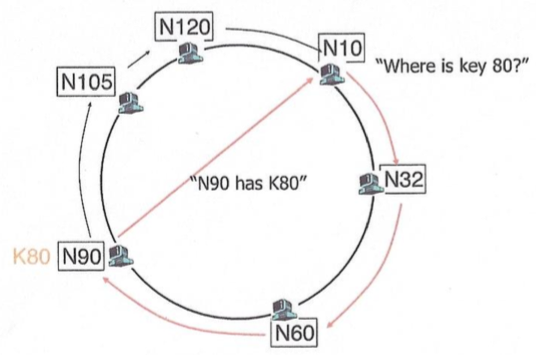
\includegraphics[width=\textwidth]{img/ch05-chord.png}
\caption{Chord Protocol}
\label{fig:ch05-chord}
\end{figure}

\paragraph{Structure}
Given $m$ bit keys, there are $2^m$ logical positions on the ring. Each host can occupy one position.

\paragraph{Find Hosts}
Each host maintains a finger table for successors. They are pointers to the nodes at $2^i$ away from it. The table makes it possible for a binary search on the network.

\begin{figure}
\centering
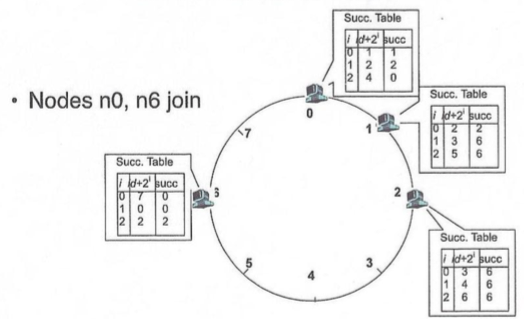
\includegraphics[width=\textwidth]{img/ch05-chord-table.png}
\caption{Chord Protocol with Suc Table}
\label{fig:ch05-chord-table}
\end{figure}

\paragraph{A Node to Join}
In order for a node to join,
\begin{enumerate}
    \item It is added to an unrepresented position.
    \item It gets its portion of the keys from its successor.
\end{enumerate}